\documentclass[letterpaper,11pt]{article}
\usepackage{../common/preamble}

% --- Variables de la portada ---
\newcommand{\tituloPractica}{Tarea 01}
\newcommand{\nombrePractica}{Diseño, simulación y comparación de filtros activos: Butterworth, Chebyshev y Bessel}
\newcommand{\fechaEntrega}{10 de Octubre de 2026}

\begin{document}

	% common/portada.tex
\thispagestyle{empty} 

\begin{center}
	\vspace{0.8cm}
	
	% --- Logo Header ---
	\begin{minipage}{0.15\textwidth}
		\centering
		\includegraphics[width=\textwidth]{UNAM\_INGENIERIA} 
	\end{minipage}
	\hfill
	\begin{minipage}{0.65\textwidth}
		\centering
		{\color{black}\fontsize{16}{18}\selectfont
			\textbf{UNIVERSIDAD NACIONAL AUTÓNOMA DE MÉXICO} \\
			\vspace{0.3cm}
			\textbf{FACULTAD DE INGENIERÍA} \\
			\vspace{0.3cm}
			\textbf{SISTEMAS DE COMUNICACIÓN} \\
			\vspace{0.3cm}
		}
	\end{minipage}
	\hfill
	\begin{minipage}{0.15\textwidth}
		\centering
		\includegraphics[width=\textwidth]{UNAM}
	\end{minipage}
	
	\vspace{1.5cm}
	
	
	\begin{tikzpicture}
		\draw[unamgold, line width=1.5pt] (0,0) -- (0.3\textwidth,0);
		\draw[unamblue, line width=1.5pt] (0.3\textwidth,0) -- (0.99\textwidth,0); 
	\end{tikzpicture}
	
	\vspace{1cm}
	
	\begin{flushright}
		
		{\color{black}\fontsize{18}{20}\selectfont
			\textbf{\MakeUppercase{\tituloPractica}} \\
			\vspace{0.6cm}
			\textbf{\MakeUppercase{\nombrePractica}}
		}
	
	\end{flushright}
	
	\vspace{1cm}
	
	\begin{flushleft}
	
		{\color{black}\fontsize{13}{15}\selectfont
		\renewcommand{\arraystretch}{1.5} % Spacing for the table
		\begin{tabular}{l l}
			\textbf{INTEGRANTES:}    & Carrasco Quiñones Diego Alexander \\
			& Díaz Antúnez David \\
			
			\textbf{GRUPO DE LABORATORIO:}       & 03 \\
			\textbf{GRUPO DE TEORÍA:}          & 07\\
			\textbf{SEMESTRE:} & 2027-1 \\
			\textbf{FECHA DE ENTREGA:} & \fechaEntrega 
    \end{tabular}
	}
		
	\end{flushleft}

	
	\vfill
	
	% --- Footer ---
	{\color{black}\fontsize{11}{13}\selectfont
		\textbf{Ciudad Universitaria, CDMX} \hfill \textbf{\fechaEntrega}
	}
\end{center}

\newpage


	\tableofcontents
	\newpage

	% ============================================================
% Filtros Pasa-bajas (Low-Pass)
% ============================================================
\section{Filtros Pasa-bajas (Low-Pass)}

\subsection{Butterworth}

\begin{figure}[H]
	\centering
	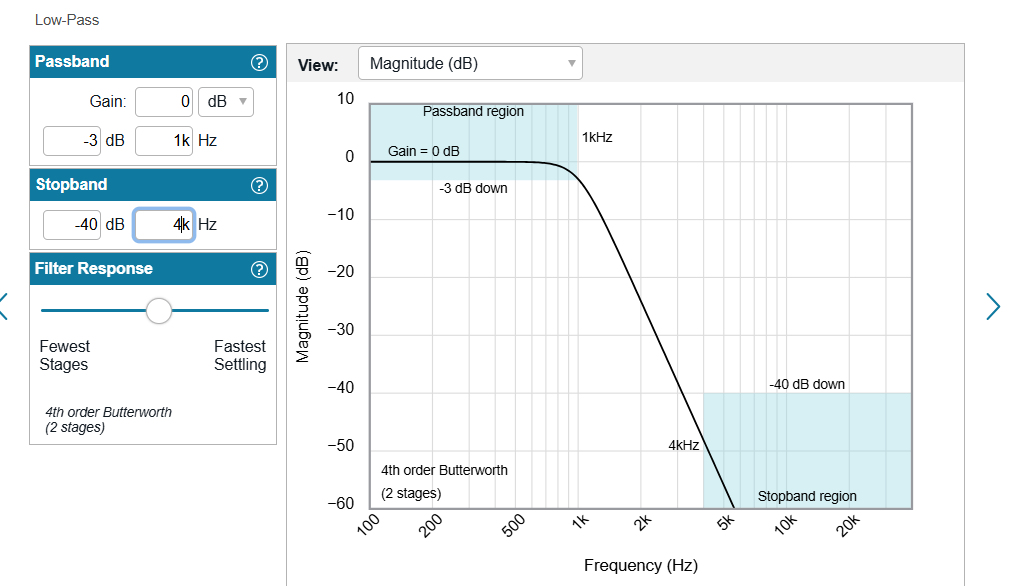
\includegraphics[width=0.9\textwidth]{img/lp_butterworth_respuesta.png}
\end{figure}

\begin{table}[H]
	\centering
	\renewcommand{\arraystretch}{1.2}
	\begin{tabular}{|l|l|}
		\hline
		\textbf{Parámetro} & \textbf{Nuestro diseño} \\
		\hline
		Tipo & Pasa-bajas \\
		Respuesta & Butterworth \\
		Orden & 4.\textsuperscript{o} \\
		Etapas & 2 \\
		Ganancia & 0\,dB \\
		Atenuación banda pasante & $-3$\,dB \\
		Frecuencia banda pasante & 1\,kHz \\
		Atenuación banda rechazo & $-40$\,dB \\
		Frecuencia banda rechazo & 4\,kHz \\
		\hline
	\end{tabular}
\end{table}

\textbf{STAGES}

\begin{figure}[H]
	\centering
	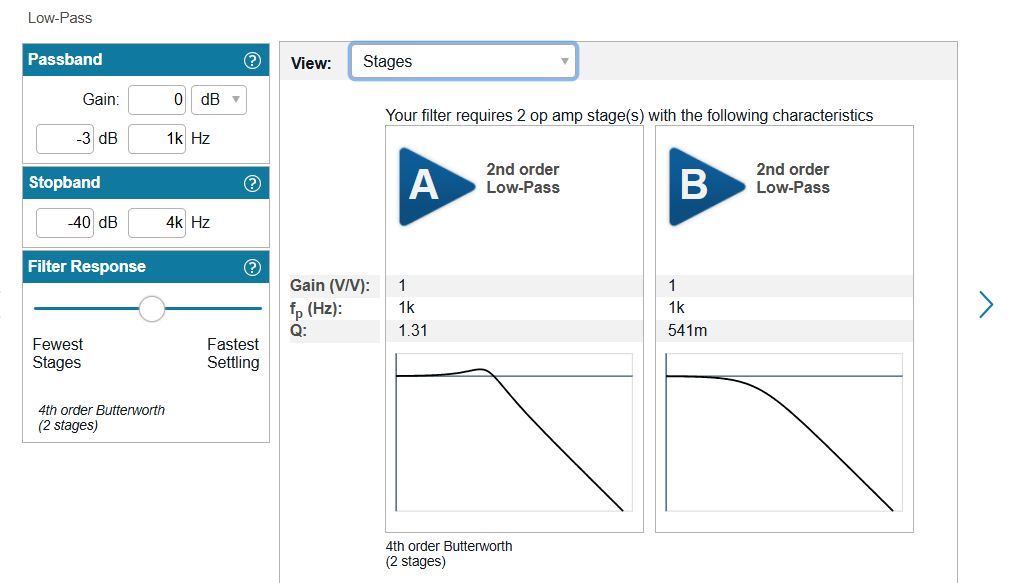
\includegraphics[width=0.9\textwidth]{img/lp_butterworth_etapas.png}
\end{figure}

\subsubsection{¿Qué es Q?}

No quiero que solamente copies ese número sin saber qué significa.

El factor de calidad $Q$ describe qué tan ``selectiva'' o resonante es una etapa de segundo orden.

En un Butterworth de cuarto orden, las dos etapas no tienen necesariamente el mismo $Q$.

Aproximadamente tendremos:
\begin{equation*}
	Q_1 \approx 0.541 \qquad Q_2 \approx 1.307
\end{equation*}

Esto es normal.

\textbf{CIRCUIT}

\begin{figure}[H]
	\centering
	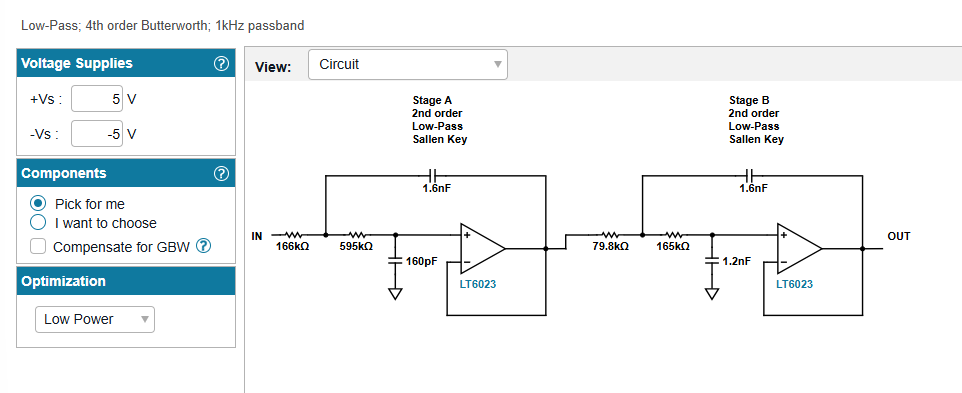
\includegraphics[width=\textwidth]{img/lp_butterworth_circuito.png}
\end{figure}

% ------------------------------------------------------------
\subsection{Chebyshev}

\begin{figure}[H]
	\centering
	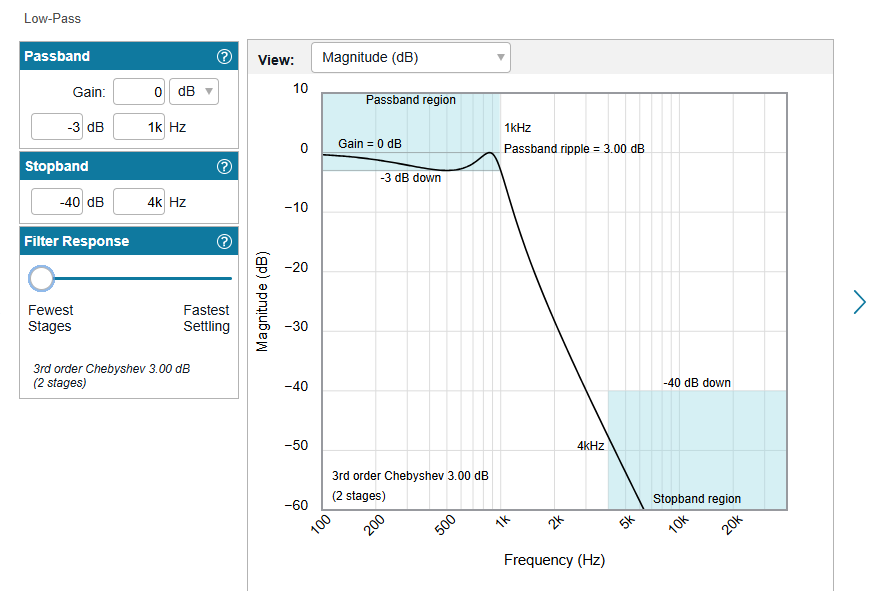
\includegraphics[width=0.9\textwidth]{img/lp_chebyshev_respuesta.png}
\end{figure}

\textbf{Stages}

\begin{figure}[H]
	\centering
	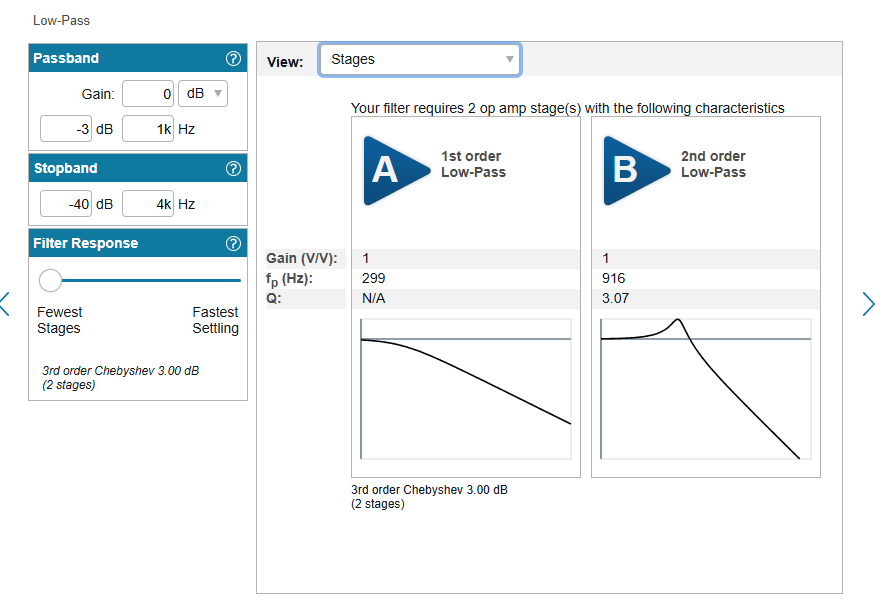
\includegraphics[width=0.9\textwidth]{img/lp_chebyshev_etapas.png}
\end{figure}

\textbf{Circuito}

\begin{figure}[H]
	\centering
	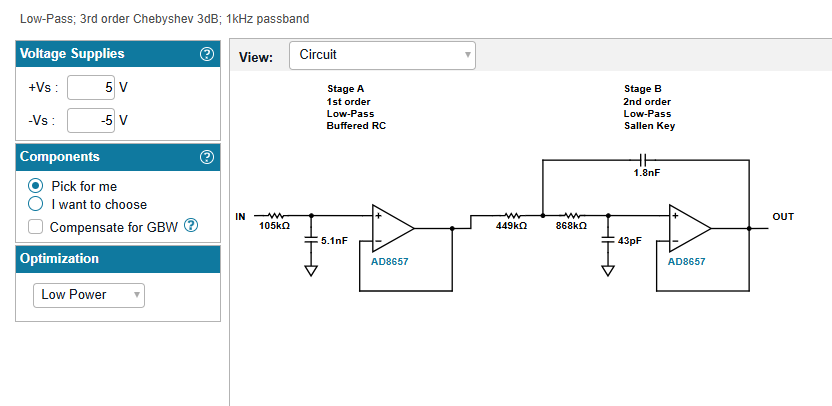
\includegraphics[width=\textwidth]{img/lp_chebyshev_circuito.png}
\end{figure}

% ------------------------------------------------------------
\subsection{Bessel}

\begin{figure}[H]
	\centering
	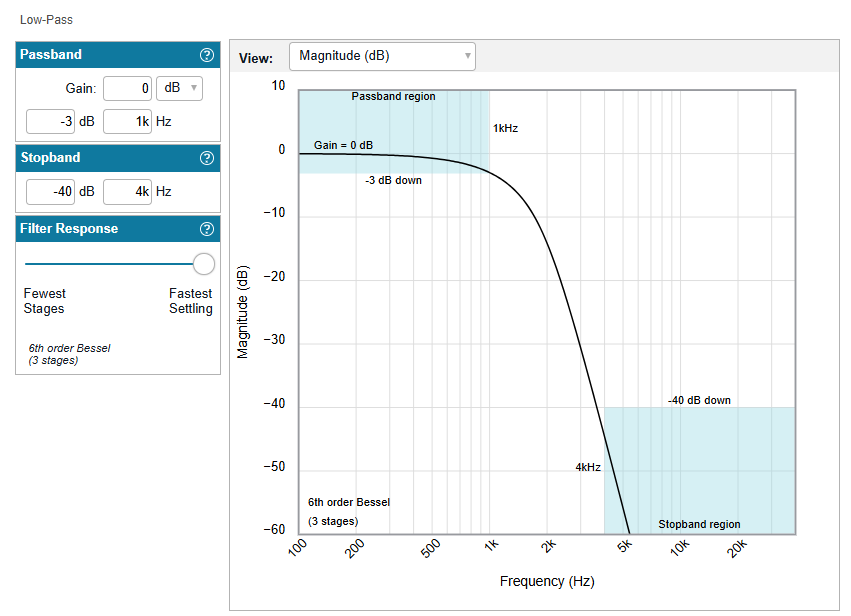
\includegraphics[width=0.9\textwidth]{img/lp_bessel_respuesta.png}
\end{figure}

\textbf{Stages}

\begin{figure}[H]
	\centering
	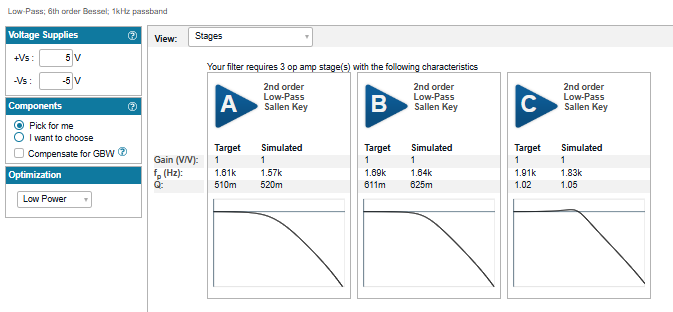
\includegraphics[width=0.9\textwidth]{img/lp_bessel_etapas.png}
\end{figure}

\textbf{Circuito}

\begin{figure}[H]
	\centering
	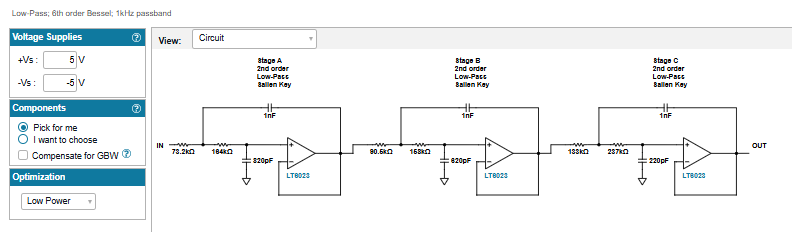
\includegraphics[width=\textwidth]{img/lp_bessel_circuito.png}
\end{figure}

	% ============================================================
% Filtros Pasa-altas (High-Pass)
% ============================================================
\section{Filtros Pasa-altas (High-Pass)}

\subsection{Butterworth}

\begin{figure}[H]
	\centering
	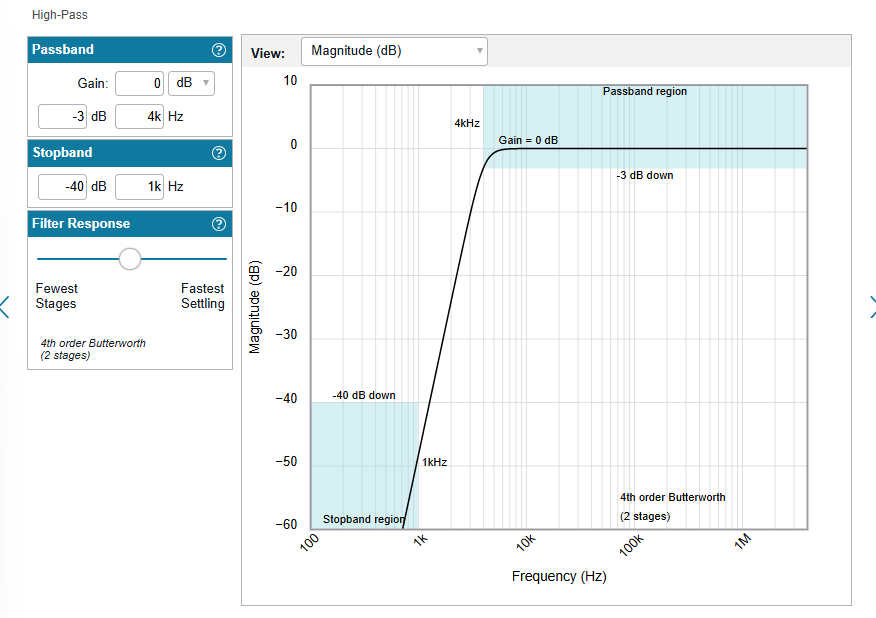
\includegraphics[width=0.9\textwidth]{img/hp_butterworth_respuesta.png}
	\caption{Respuesta en magnitud del filtro pasa-altas Butterworth de 4.\textsuperscript{o} orden.}
	\label{fig:hp_butterworth_respuesta}
\end{figure}

\begin{figure}[H]
	\centering
	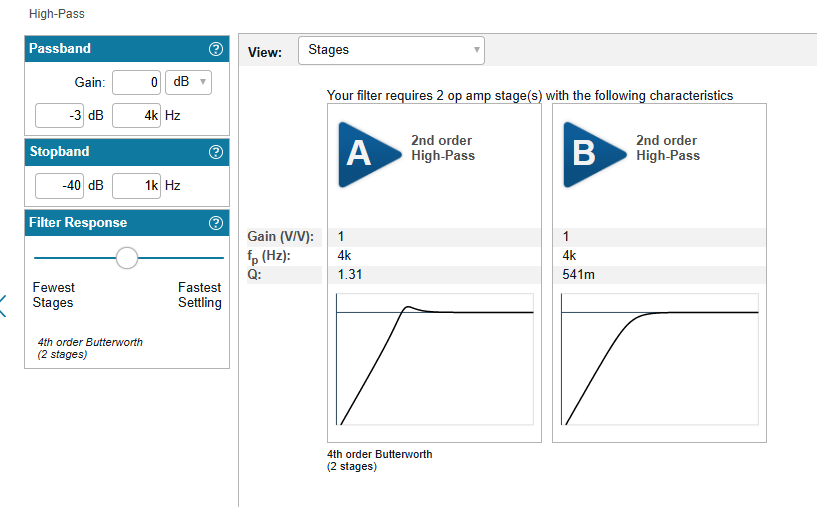
\includegraphics[width=0.9\textwidth]{img/hp_butterworth_etapas.png}
	\caption{Configuración de etapas (\textit{Stages}) del filtro pasa-altas Butterworth: dos etapas de segundo orden.}
	\label{fig:hp_butterworth_etapas}
\end{figure}

\begin{figure}[H]
	\centering
	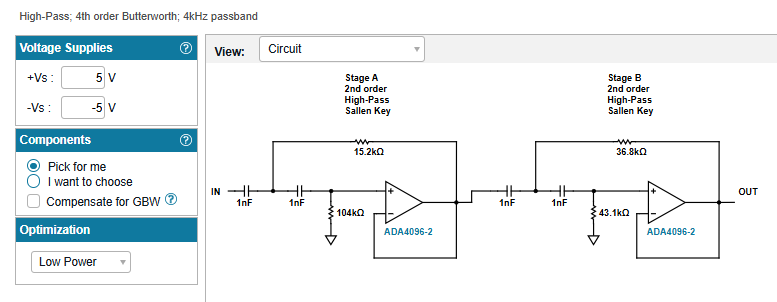
\includegraphics[width=\textwidth]{img/hp_butterworth_circuito.png}
	\caption{Circuito del filtro pasa-altas Butterworth.}
	\label{fig:hp_butterworth_circuito}
\end{figure}

% ------------------------------------------------------------
\subsection{Chebyshev}

\begin{figure}[H]
	\centering
	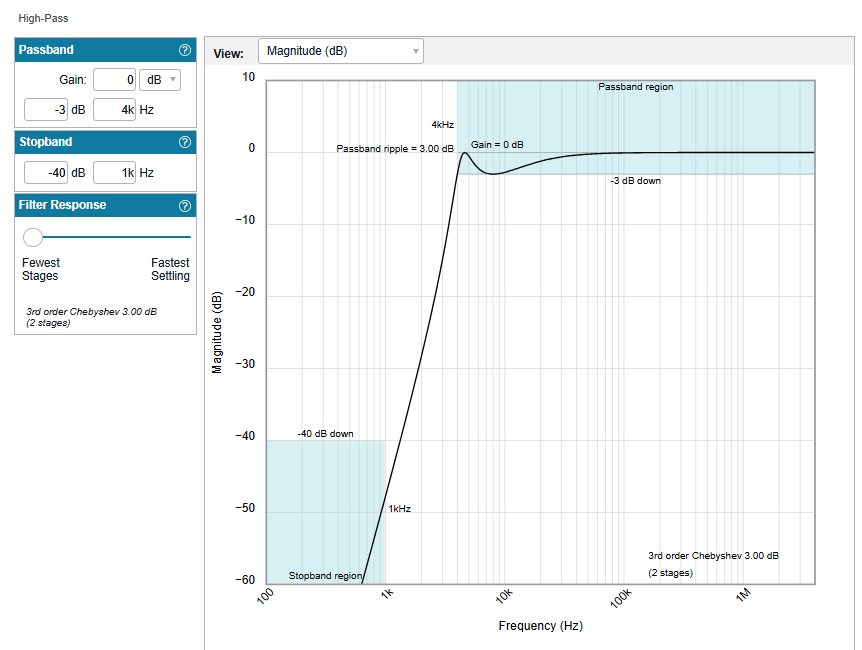
\includegraphics[width=0.9\textwidth]{img/hp_chebyshev_respuesta.png}
	\caption{Respuesta en magnitud del filtro pasa-altas Chebyshev de 3.\textsuperscript{er} orden (rizo de 3\,dB en la banda de paso).}
	\label{fig:hp_chebyshev_respuesta}
\end{figure}

\begin{figure}[H]
	\centering
	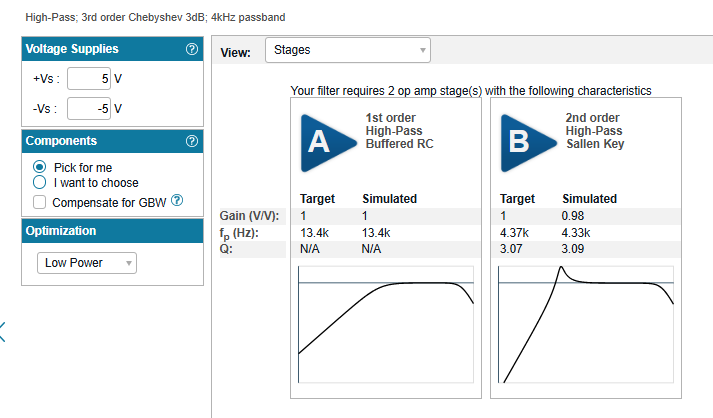
\includegraphics[width=0.9\textwidth]{img/hp_chebyshev_etapas.png}
	\caption{Configuración de etapas (\textit{Stages}) del filtro pasa-altas Chebyshev.}
	\label{fig:hp_chebyshev_etapas}
\end{figure}

\begin{figure}[H]
	\centering
	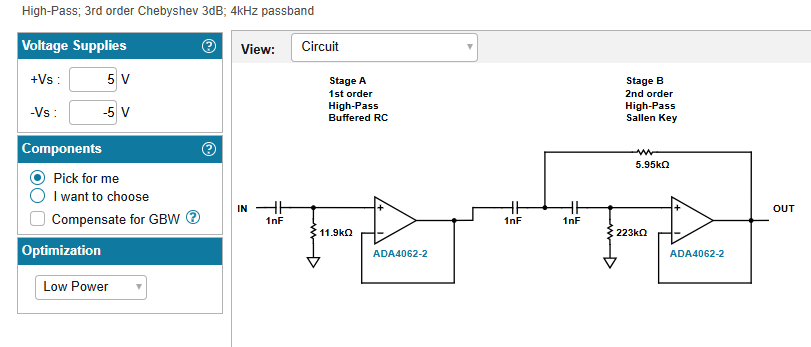
\includegraphics[width=\textwidth]{img/hp_chebyshev_circuito.png}
	\caption{Circuito del filtro pasa-altas Chebyshev.}
	\label{fig:hp_chebyshev_circuito}
\end{figure}

% ------------------------------------------------------------
\subsection{Bessel}

\begin{figure}[H]
	\centering
	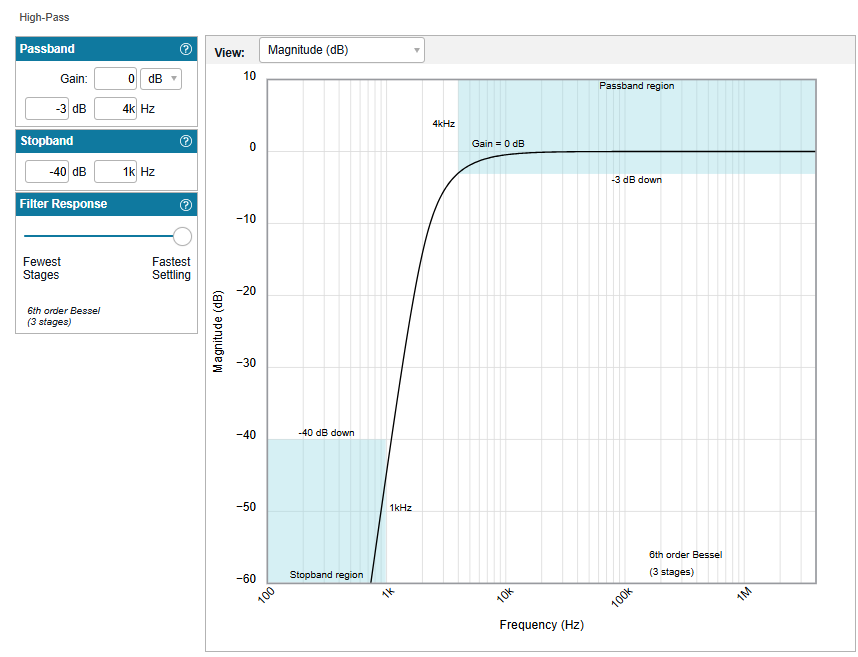
\includegraphics[width=0.9\textwidth]{img/hp_bessel_respuesta.png}
	\caption{Respuesta en magnitud del filtro pasa-altas Bessel de 6.\textsuperscript{o} orden.}
	\label{fig:hp_bessel_respuesta}
\end{figure}

\begin{figure}[H]
	\centering
	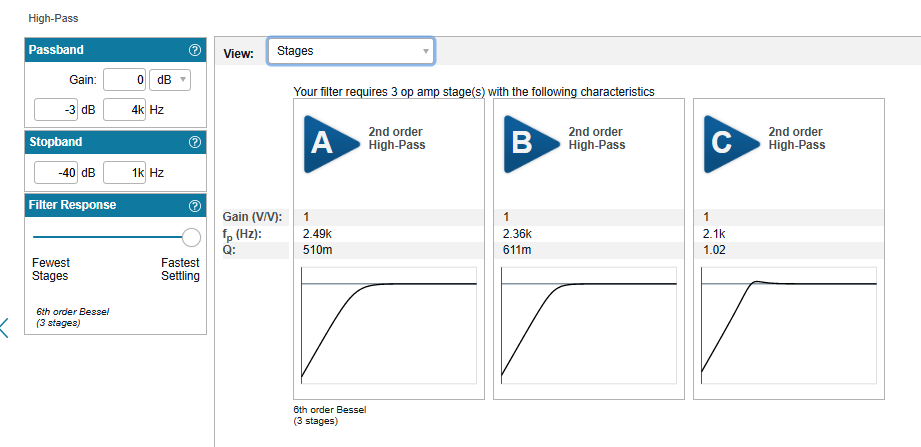
\includegraphics[width=0.9\textwidth]{img/hp_bessel_etapas.png}
	\caption{Configuración de etapas (\textit{Stages}) del filtro pasa-altas Bessel: tres etapas de segundo orden.}
	\label{fig:hp_bessel_etapas}
\end{figure}

\begin{figure}[H]
	\centering
	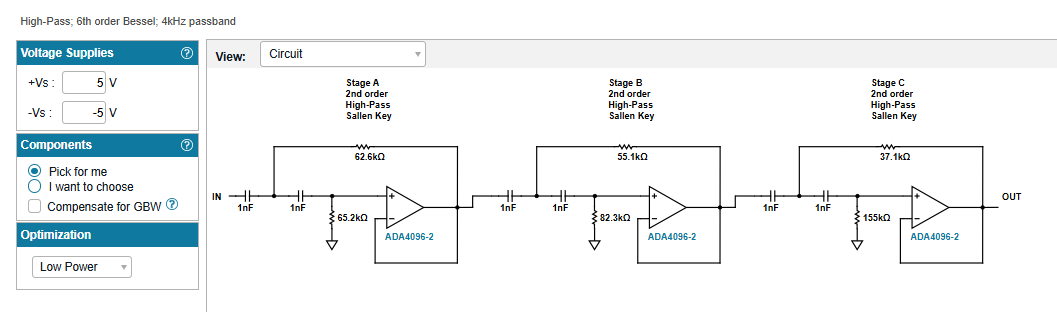
\includegraphics[width=\textwidth]{img/hp_bessel_circuito.png}
	\caption{Circuito del filtro pasa-altas Bessel.}
	\label{fig:hp_bessel_circuito}
\end{figure}

	% ============================================================
% Filtros Pasa-banda (Band-Pass)
% ============================================================
\section{Filtros Pasa-banda (Band-Pass)}

\subsection{Butterworth}

\begin{figure}[H]
	\centering
	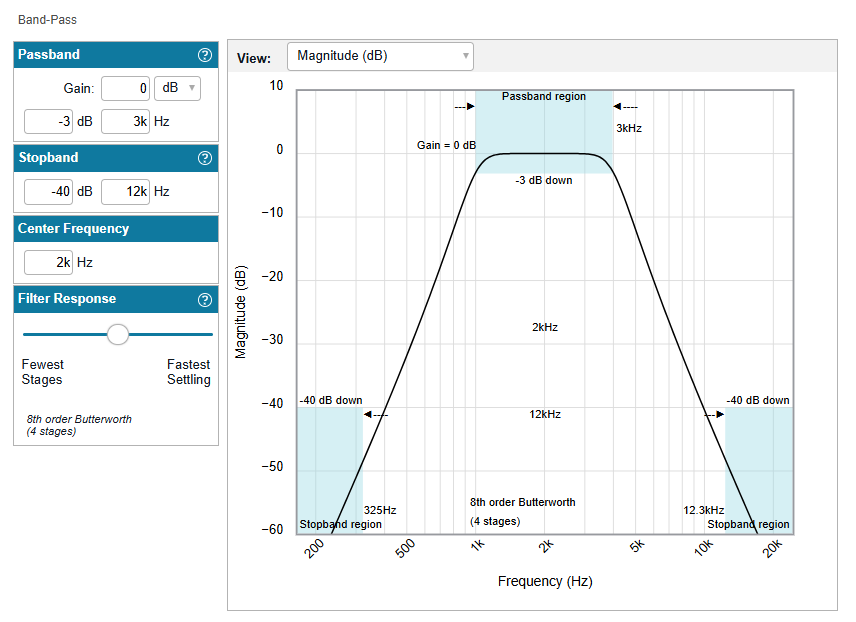
\includegraphics[width=0.9\textwidth]{img/bp_butterworth_respuesta.png}
	\caption{Respuesta en magnitud del filtro pasa-banda Butterworth de 8.\textsuperscript{o} orden (centrado en 2\,kHz).}
	\label{fig:bp_butterworth_respuesta}
\end{figure}

\begin{figure}[H]
	\centering
	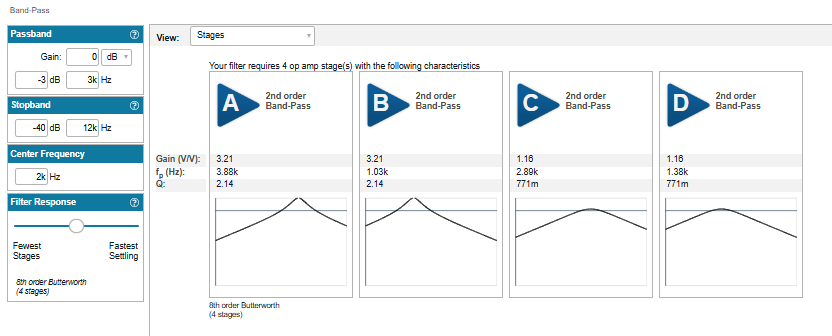
\includegraphics[width=0.9\textwidth]{img/bp_butterworth_etapas.png}
	\caption{Configuración de etapas (\textit{Stages}) del filtro pasa-banda Butterworth: cuatro etapas de segundo orden.}
	\label{fig:bp_butterworth_etapas}
\end{figure}

\begin{figure}[H]
	\centering
	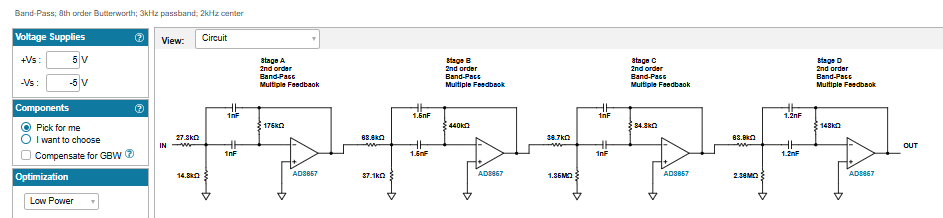
\includegraphics[width=\textwidth]{img/bp_butterworth_circuito.png}
	\caption{Circuito del filtro pasa-banda Butterworth.}
	\label{fig:bp_butterworth_circuito}
\end{figure}

% ------------------------------------------------------------
\subsection{Chebyshev}

\begin{figure}[H]
	\centering
	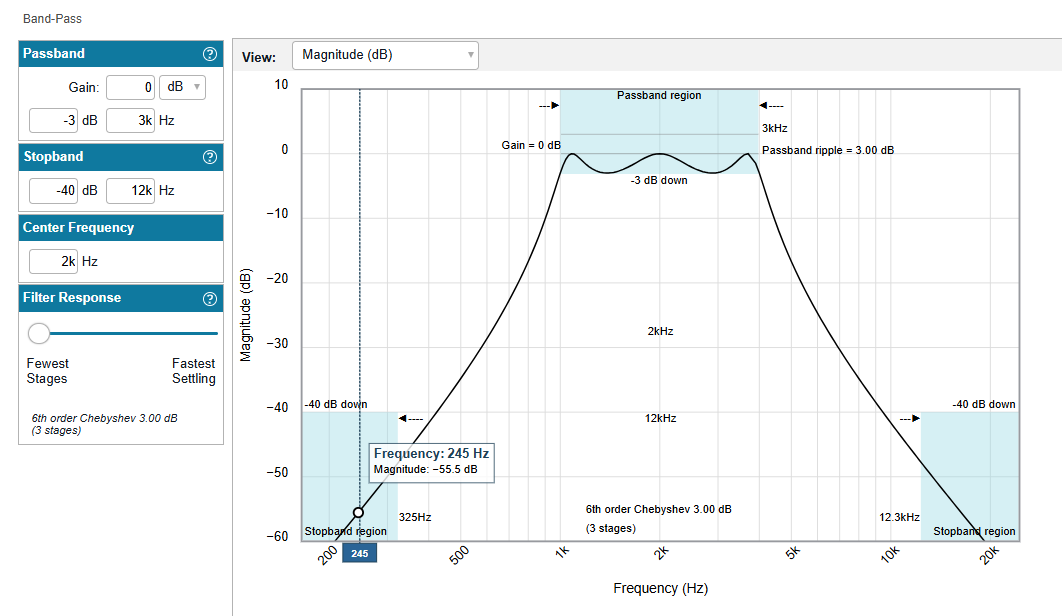
\includegraphics[width=0.9\textwidth]{img/bp_chebyshev_respuesta.png}
	\caption{Respuesta en magnitud del filtro pasa-banda Chebyshev de 6.\textsuperscript{o} orden (rizo de 3\,dB, centrado en 2\,kHz).}
	\label{fig:bp_chebyshev_respuesta}
\end{figure}

\begin{figure}[H]
	\centering
	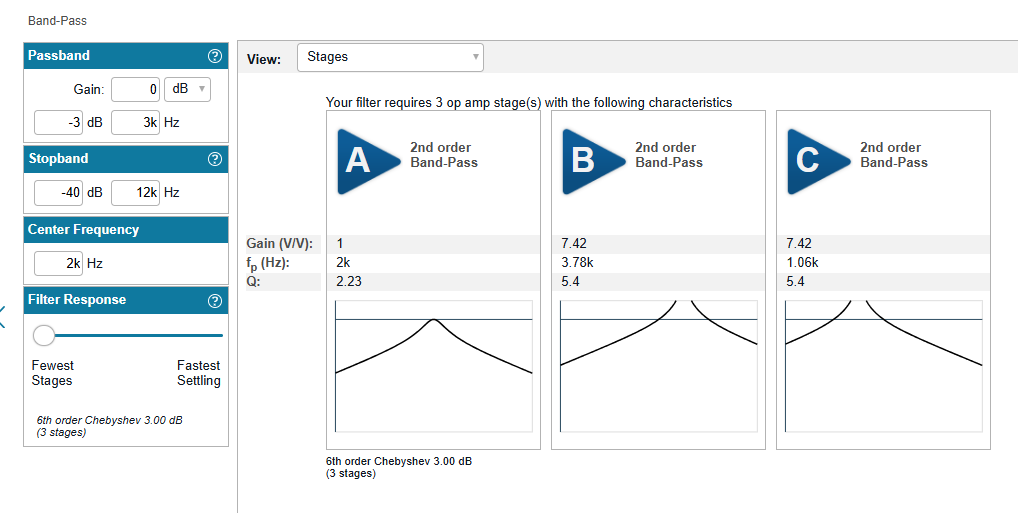
\includegraphics[width=0.9\textwidth]{img/bp_chebyshev_etapas.png}
	\caption{Configuración de etapas (\textit{Stages}) del filtro pasa-banda Chebyshev: tres etapas de segundo orden.}
	\label{fig:bp_chebyshev_etapas}
\end{figure}

\begin{figure}[H]
	\centering
	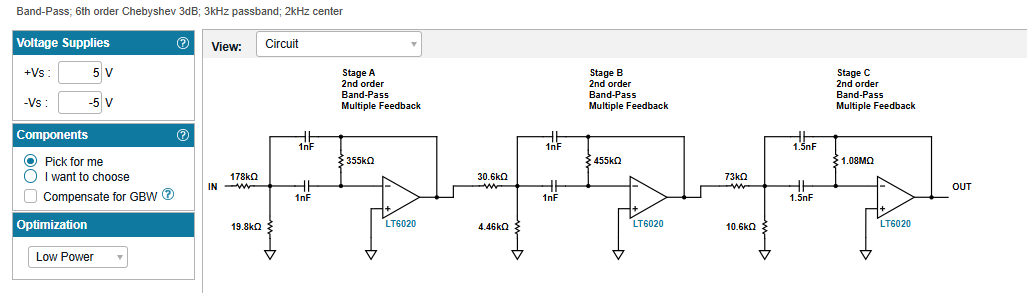
\includegraphics[width=\textwidth]{img/bp_chebyshev_circuito.png}
	\caption{Circuito del filtro pasa-banda Chebyshev.}
	\label{fig:bp_chebyshev_circuito}
\end{figure}

% ------------------------------------------------------------
\subsection{Bessel}

\begin{figure}[H]
	\centering
	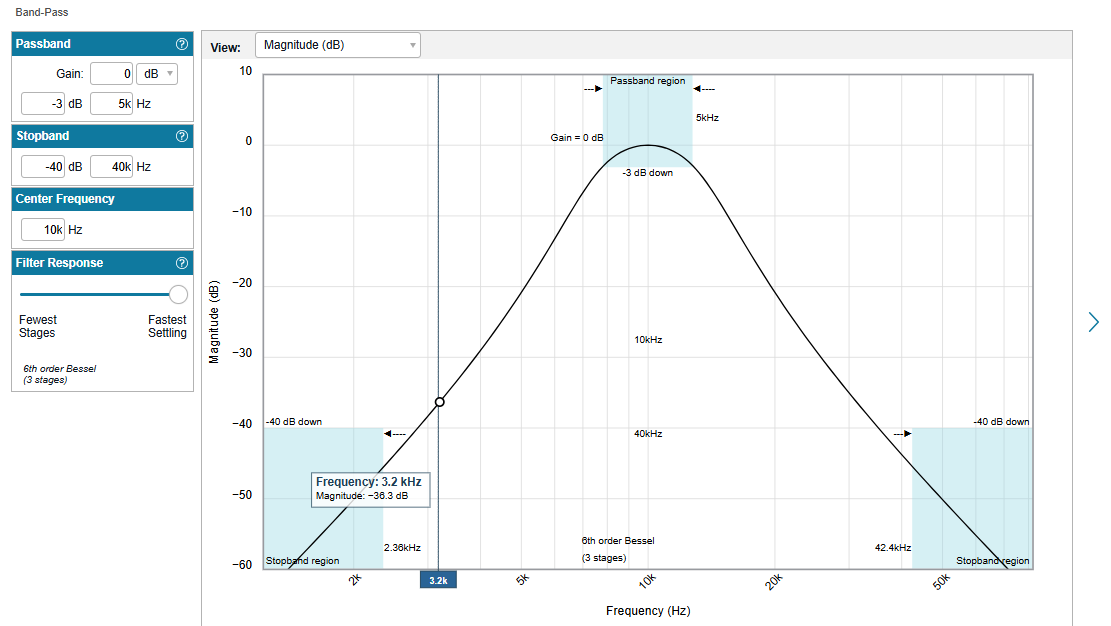
\includegraphics[width=0.9\textwidth]{img/bp_bessel_respuesta.png}
	\caption{Respuesta en magnitud del filtro pasa-banda Bessel de 6.\textsuperscript{o} orden (centrado en 10\,kHz).}
	\label{fig:bp_bessel_respuesta}
\end{figure}

\begin{figure}[H]
	\centering
	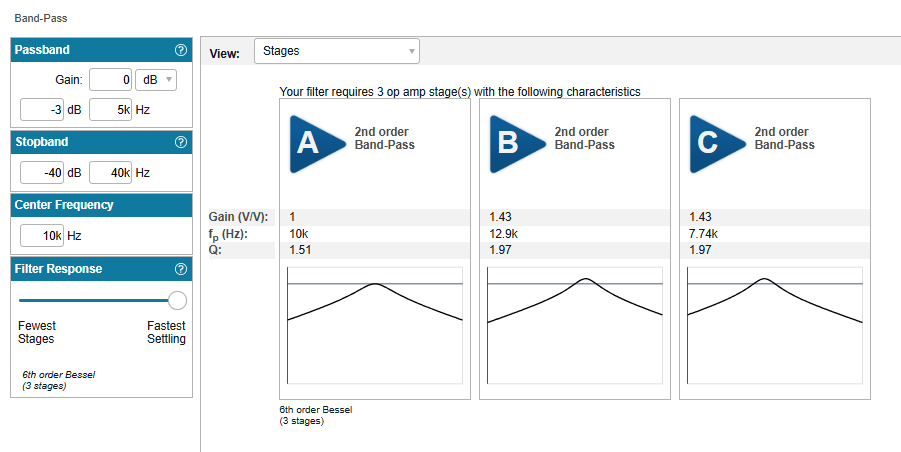
\includegraphics[width=0.9\textwidth]{img/bp_bessel_etapas.png}
	\caption{Configuración de etapas (\textit{Stages}) del filtro pasa-banda Bessel: tres etapas de segundo orden.}
	\label{fig:bp_bessel_etapas}
\end{figure}

\begin{figure}[H]
	\centering
	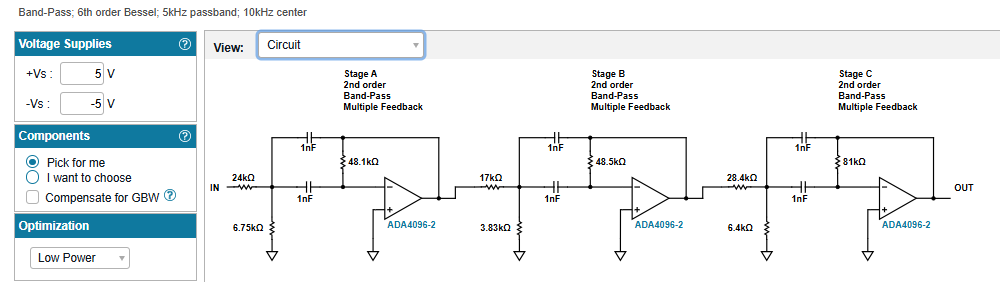
\includegraphics[width=\textwidth]{img/bp_bessel_circuito.png}
	\caption{Circuito del filtro pasa-banda Bessel.}
	\label{fig:bp_bessel_circuito}
\end{figure}

	% ============================================================
% Preguntas de análisis
% ============================================================
\section{Pregunta 1: ¿Qué diferencias existen entre el Filtro Paso Altas, Filtro Paso Bajas y Filtro Paso Banda?}

Basándonos en la configuración de parámetros y la forma de la respuesta en frecuencia observada en las gráficas de simulación:

\begin{itemize}
	\item \textbf{Filtro Paso Bajas (Low-Pass):}
	\begin{itemize}
		\item \textbf{Comportamiento simulado:} Deja pasar la señal limpia a $0$\,dB desde $0$\,Hz hasta la frecuencia de paso de $1$\,kHz (Banda de Paso). A partir de ahí, la magnitud disminuye gradualmente hasta alcanzar una atenuación de $-40$\,dB a los $4$\,kHz (Banda de Atenuación).
		\item \textbf{Función:} Elimina componentes de alta frecuencia y ruido, dejando intactas las frecuencias bajas.
	\end{itemize}
	\item \textbf{Filtro Paso Altas (High-Pass):}
	\begin{itemize}
		\item \textbf{Comportamiento simulado:} Bloquea las frecuencias bajas (atenuación de $-40$\,dB de $0$\,Hz hasta $1$\,kHz) y permite el paso libre a $0$\,dB a partir de $4$\,kHz hacia adelante.
		\item \textbf{Función:} Elimina componentes continuas (DC) o ruidos de baja frecuencia, dejando pasar únicamente las componentes de alta frecuencia.
	\end{itemize}
	\item \textbf{Filtro Paso Banda (Band-Pass):}
	\begin{itemize}
		\item \textbf{Comportamiento simulado:} Combina ambas acciones definiendo un ancho de banda útil de $3$\,kHz centrado en $2$\,kHz. Mantiene la ganancia en $0$\,dB en el centro y atenuación de $-40$\,dB tanto hacia frecuencias bajas ($325$\,Hz) como hacia frecuencias altas ($12.3$\,kHz).
		\item \textbf{Función:} Delimita una ventana específica de frecuencias de interés y rechaza todo lo que quede por encima o por debajo de esta banda.
	\end{itemize}
\end{itemize}

\section{Pregunta 2: ¿Qué diferencias existen entre el Filtro Butterworth, Chebyshev y Bessel?}

A partir de la comparación del comportamiento del circuito y el número de etapas requeridas (\textit{stages}) registrado por el simulador:

\begin{table}[H]
	\centering
	\footnotesize
	\renewcommand{\arraystretch}{1.3}
	\begin{tabular}{|p{2.3cm}|p{4.4cm}|p{4.4cm}|p{4.4cm}|}
		\hline
		\textbf{Característica} & \textbf{Butterworth} & \textbf{Chebyshev} & \textbf{Bessel} \\
		\hline
		Respuesta en la banda de paso & Máxima planitud: la ganancia se mantiene plana, sin rizado, antes de la frecuencia de corte. & Presenta ondulaciones o rizado (ripple) en la banda de paso, a cambio de una transición más rápida. & Presenta una caída más suave y redondeada cerca de la frecuencia de corte. \\
		\hline
		Velocidad de caída (pendiente) & Caída uniforme y selectividad intermedia. & Transición más rápida y abrupta entre la banda de paso y la banda de atenuación, para un mismo orden. & Transición más lenta y gradual hacia la zona de atenuación. \\
		\hline
		Respuesta en el tiempo y fase & Respuesta de fase moderada; puede presentar cierto sobretiro ante señales transitorias. & Menor linealidad de fase; puede introducir más distorsión en la forma de onda temporal. & Excelente linealidad de fase y retardo de grupo aproximadamente constante en la banda de interés. Conserva mejor la forma de onda. \\
		\hline
		Orden y complejidad requerida & Puede requerir un orden intermedio para cumplir las especificaciones; por ejemplo, 4.\textsuperscript{o} orden (2 etapas) en un filtro pasa-bajas. & Puede alcanzar una atenuación determinada con un orden menor que Butterworth, dependiendo de las especificaciones y del rizado permitido. & Puede requerir un orden mayor para alcanzar la misma atenuación, debido a su transición más gradual. \\
		\hline
		Ventaja principal & Respuesta de amplitud plana en la banda de paso. & Mayor selectividad en frecuencia. & Mejor conservación de la forma de onda y de las características temporales. \\
		\hline
		Desventaja principal & Transición menos abrupta que Chebyshev. & Rizado en la banda de paso y mayor distorsión de fase. & Menor selectividad en frecuencia para un mismo orden. \\
		\hline
		Aplicaciones típicas & Audio, instrumentación y acondicionamiento general de señales. & Sistemas donde se necesita separar frecuencias con mayor rapidez. & Audio, pulsos y sistemas donde importa conservar la forma de onda. \\
		\hline
	\end{tabular}
\end{table}


\end{document}
